\section{Graphes hamiltoniens}
\subsection{Graphes hamiltoniens}
\index{chemin!chemin hamiltonien}
\begin{mydef}
  Un \emph{chemin} est \emph{hamiltonien} s’il passe par chaque noeud du graphe une et une seule fois.
\end{mydef}

\index{cycle!cycle hamiltonien}
\begin{mydef}
  Un \emph{cycle} est \emph{hamiltonien} s’il passe par chaque noeud du graphe une et une seule fois.
\end{mydef}

\index{graphe!graphe hamiltonien}
\begin{mydef}
  Un \emph{graphe} est \emph{hamiltonien} s’il possède un cycle hamiltonien.
\end{mydef}

\begin{mytheo} [Condition nécessaire pour un graphe hamiltonien]
  Si on ôte $k$ noeuds quelconques d’un graphe hamiltonien, on obtient au plus $k$ composantes connexes.
  \begin{proof}
     Soit $v_1 ... v_nv_1$, le cycle hamiltonien.\\
     Retirer $k$ noeuds du cycle laisse $\leq k$ composantes (=morceaux du cycle connexes), on crée au plus $k$ chemins, tous les noeuds sur un même chemin sont dans une même composante connexe. Les autres arêtes ne peuvent que diminuer encore le nombre de composantes connexes.
  \end{proof}
\end{mytheo}
\begin{myexem} Le graphe suivant est bien hamiltonien.
  \begin{figure} [!h]
      \hspace*{\fill}
         \subfigure[]
         {
             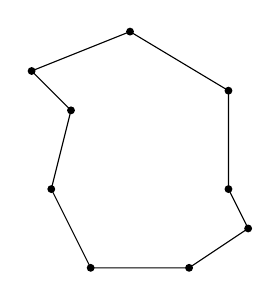
\begin{tikzpicture}[scale = 0.5]
          	 \fill[black] (-1,0) circle (0.1cm);
          	 \fill[black] (-2,2) circle (0.1cm);
          	 \fill[black] (-1.5,4) circle (0.1cm);
          	 \fill[black] (-2.5,5) circle (0.1cm);
          	 \fill[black] (0,6) circle (0.1cm);
          	 \fill[black] (2.5,4.5) circle (0.1cm);
          	 \fill[black] (2.5,2) circle (0.1cm);
          	 \fill[black] (3,1) circle (0.1cm);
          	 \fill[black] (1.5,0) circle (0.1cm);

          	 \draw (-1,0) -- (-2,2) -- (-1.5,4) -- (-2.5,5) -- (0,6) -- (2.5,4.5) -- (2.5,2) -- (3,1) -- (1.5,0) -- cycle;
        \end{tikzpicture}
      	}
      	\hfill
      \subfigure[] 
         {
             \begin{tikzpicture}[scale = 0.5]
          	 \fill[black] (-1,0) circle (0.1cm);
          	 \fill[black] (-2,2) circle (0.1cm);
          	 \fill[black] (-2.5,5) circle (0.1cm);
          	 \fill[black] (0,6) circle (0.1cm);
          	 \fill[black] (2.5,2) circle (0.1cm);
          	 \fill[black] (3,1) circle (0.1cm);

             \draw (-2.5,5) -- (0,6);
          	 \draw (-1,0) -- (-2,2);
          	 \draw (2.5,2) -- (3,1);
        \end{tikzpicture}
      	}
      	\hspace*{\fill}
    \end{figure} \newline
    En retirant 3 noeuds du graphe $g$ on obtient bien 3 composantes connexes dans le graphe $h$.
\end{myexem}

\begin{mytheo} [Condition suffisante pour un graphe hamiltonien]
  Un graphe simple à $n \geq 3$ noeuds tel que le degré minimum est d’au moins $n/2$ est hamiltonien.
  \begin{proof}
     Par l'absurde.

     Supposons qu'il existe un graphe à $n \geq 3$ noeuds de degré minimum $d(v) \geq \frac{n}{2}$ non hamiltonien.

     Prenons un tel graphe qui est maximal pour cette propriété : ajouter une arête dans ce graphe le rendrait hamiltonien.

     Ce graphe G n'est pas le graphe complet $K_n$
     \begin{align*}
		&\Rightarrow \exists \text{ des noeuds } v_1, v_n \text{ non adjacents} \\
		&\Rightarrow G + \{v_1, v_n \} \text{ est hamiltonien} \\
		&\Rightarrow \exists \text{ un cycle hamiltonien passant par l'arête } v_1v_n \\
		&\Rightarrow \text{Dans } G, \exists \text{ un chemin hamiltonien } v_1v_2...v_n
	\end{align*}
	Considérons les ensembles:
	\begin{align*}
		S &= \{v_i \mid v_{i+1} \text{ est adjacent à } v_1\} &\vert S \vert = \text{degré}(v_1) \geq \frac{n}{2}\\
		T &= \{v_i \mid v_{i} \text{ est adjacent à } v_n\} &\vert T \vert = \text{degré}(v_n) \geq \frac{n}{2}
	\end{align*}
	On sait que $v_n \not\in S$, par hypothèse $v_1$ et $v_n$ ne sont pas adjacents, et $v_n \not\in T$. On a donc $\vert S \cup T \vert < n$ puisqu'aucun des ensembles ne contient $v_n$.
	De plus, $\vert S \cap T \vert = \emptyset $ : en effet, si $\exists v_i \in \vert S \cap T \vert$, alors $v_1v_2...v_iv_nv_{n-1}...v_{i+1}v_1$ est un cycle hamiltonien $\Rightarrow$ Contradiction
	\begin{figure} [!h]
		\center
        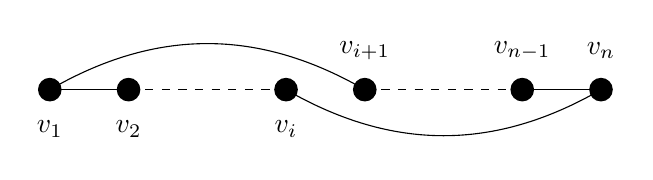
\begin{tikzpicture}[scale = 0.5]
          	 \fill[black] (-7,0) circle (0.3cm);
          	 \node at (-7,-1) {$v_1$};
          	 \fill[black] (-5,0) circle (0.3cm);
          	 \node at (-5,-1) {$v_2$};
          	 \fill[black] (-1,0) circle (0.3cm);
          	 \node at (-1,-1) {$v_i$};
          	 \fill[black] (1,0) circle (0.3cm);
          	 \node at (1,1) {$v_{i+1}$};
          	 \fill[black] (5,0) circle (0.3cm);
          	 \node at (5,1) {$v_{n-1}$};
          	 \fill[black] (7,0) circle (0.3cm);
          	 \node at (7,1) {$v_n$};

          	 \draw (-7,0) -- (-5,0);
          	 \draw [dashed] (-5,0) -- (-1,0);
          	 \draw [dashed] (1,0) -- (5,0);
          	 \draw (5,0) -- (7,0);
          	 \draw (1,0) to[bend right] (-7,0);
          	 \draw (-1,0) to[bend right] (7,0);
        \end{tikzpicture}
    \end{figure}
	\newline \newline
	Enfin, $\vert S \cup T \vert = \vert S \vert + \vert T \vert - \vert S \cap T \vert \geq n$ mais $\vert S \cup T \vert < n$ $\Rightarrow$ Contradiction
  \end{proof}
\end{mytheo}

\index{problème}
\index{problème!du postier chinois}
\begin{mydef} [Problème du postier chinois]
  Dans un graphe pondéré, trouver le parcours fermé le plus court qui passe par toutes les arêtes au moins une fois.
\end{mydef}

\index{problème!du voyageur de commerce}
\begin{mydef} [Problème du voyageur de commerce]
  Dans un graphe pondéré, trouver le parcours fermé le plus court qui passe par tous les noeuds au moins une fois.
\end{mydef}
